\documentclass[a4paper, twoside, 10pt]{article}
\usepackage[dutch]{babel}
\usepackage{cleveref}
\usepackage{listings}			% Used to include VHDL-code and fragments
\usepackage{graphicx}			% Used to include .pdf, .jpg and .png-files
\usepackage{eso-pic}			% Absolute positioning, lines-to-track appendix and front- and backpage
\usepackage{verbatim}			% For comment-environment
\usepackage{enumitem}			% Mogelijkheid tot geen enters in itemize en enurate

\crefname{equation}{vergelijking}{vergelijkingen}
\crefname{table}{tabel}{tabellen}
\crefname{figure}{figuur}{figuren}

\definecolor{comment}{RGB}{0, 15 , 117}		%Kleur blauw defineren
\definecolor{keyword}{RGB}{165, 42, 42}		%Kleur rood defineren
\definecolor{STD}{RGB}{46, 139, 87}			%Kleur groen defineren

\lstdefinelanguage{VHDL}{
  morekeywords=[1]{ 						%Defineren van keywords die blauw worden
    library,use,all,entity,is,port,in,out,end,architecture,of,
    begin,and,or,not,downto,ALL,signal,type,case,if,elsif,for,when,array,
    others,loop,process,to},
  morekeywords=[2]{							%Defineren van keyword die groen worden
    STD_LOGIC_VECTOR,STD_LOGIC,STD_LOGIC_1164,
    NUMERIC_STD,STD_LOGIC_ARITH,STD_LOGIC_UNSIGNED,std_logic_vector,unsigned,
    std_logic},
  morecomment=[l]--}
  
\lstdefinestyle{vhdl}{
  language     = VHDL,
  basicstyle   = \footnotesize \ttfamily,
  keywordstyle = [1]\color{keyword}\bfseries, 	% Keywords kleuren
  keywordstyle = [2]\color{STD}\bfseries,		% Keywords kleuren
  commentstyle = \color{comment},				% Comments kleuren
  numbers=left,					 				% Regel nummering
  breaklines=true,               				% sets automatic line breaking
  tabsize=4                     				% sets default tabsize to 4 spaces
}

\begin{document}

\section{Functionaliteit}
Het DCF blok dient volgens de specificaties een tijd- en dagstempel te genereren uit het gedigitaliseerde DCF77 signaal dat aan het blok wordt aangeboden. Bovendien dient het blok de tijd zelf bij te houden wanneer het DCF77 signaal niet of niet goed wordt ontvangen. Het is vrij ondoenlijk om deze volledige functionaliteit in \'e\'en keer te implementeren in VHDL. Bovendien zou dit een groot, lomp blok opleveren in de layout, welke vervolgens lastig op de chip te plaatsen zal zijn. Daarom wordt het DCF blok opgedeeld in kleinere subblokken, welke vervolgens wel in \'e\'en keer geïmplementeerd kunnen worden. Een top-level beschrijving knoopt vervolgens de kleinere subblokken weer aan elkaar tot een groot blok. Naast het voordeel dat dit het ontwerpen vergemakkelijkt, geeft dit ook een veel beter op de chip te plaatsen ontwerp, omdat ook de layout op dezelfde hi\"erarchische manier gegenereerd zal worden.\\

\noindent In \cref{fig: dcf_subblokken} is te zien hoe het DCF blok is verdeeld in subblokken. Het DCF77 signaal wordt allereerst aangeboden aan het subblok edge detector, welke dit signaal vervolgens opsplitst in twee afzonderlijke signalen. Het eerste signaal geeft een puls wanneer er een rising edge plaatsvind op het DCF77 signaal en het tweede signaal geeft een puls wanneer er een falling edge plaatsvind op het DCF77 signaal. Beide signalen worden doorgevoerd naar de daadwerkelijke DCF decoder, welke aan de hand van het tijdsverschil tussen de rising en falling edges bepaald wat de bitreeks is die in \'e\'en minuut van het DCF77 signaal gecodeerd is. Uit deze bitreeks worden vervolgens de gewenste bits geselecteerd en vervolgens naar buiten gevoerd. Naast deze bits genereerd het decoder blok ook een debug signaal ``dcf\_led'', welke aangeeft of het DCF77 signaal goed wordt ontvangen, en een signaal ``start'' dat aangeeft wanneer een volledige minuut is gedecodeerd. Dit laatste signaal gaat, samen met de gewentste bits (inclusief parity bits), naar het subblok parity check. Hier wordt gecontroleerd of het aantal enen (even of oneven) klopt met wat het parity bit aangeeft. Het parity bit is namelijk alleen 1 wanneer er een even aantal bits bij hoort. De parity controle wordt uitgevoerd door een xor operatie te gebruiken op de relevante bits. Het subblok parity check genereert vervolgens twee signalen. \'E\'en signaal geeft aan dat de datum aan de uitgang van de decoder gebruikt kan worden en het andere geeft aan dat er met de gedecodeerde tijd verder gewerkt kan worden. Dit gebeurt vervolgens in het subblok BCD to bin, waar het BCD gecodeerde tijdsignaal uit het DCF77 signaal wordt omgezet in een binair signaal. Wanneer deze conversie afgelopen is, zal ook weer een signaal worden gegenereerd wat aan het volgende subblok aangeeft dat het kan beginnen.\\

\noindent Dit volgende subblok is de autonome synchroniseerbare klok. Dit subblok besstaat vervolgens zelf weer uit twee mod60 tellers en een mod24 teller, waarmee autonoom de tijd kan wordt bijgehouden. Wanneer het subblok BCD to bin dit aangeeft, worden deze tellers gesynchroniseerd met de tijd uit het DCF77 signaal. Voor het bijhouden van de tijd wordt gebruik gemaakt van het uitgangssignaal van een ander subblok, namelijk de klokdeler. Dit subblok genereerd een 1 Hz signaal, wat wordt gebruikt voor het tellen van seconden en bovendien naar andere blokken buiten het DCF blok wordt doorgevoerd.

\begin{figure}[ht]
\begin{center}
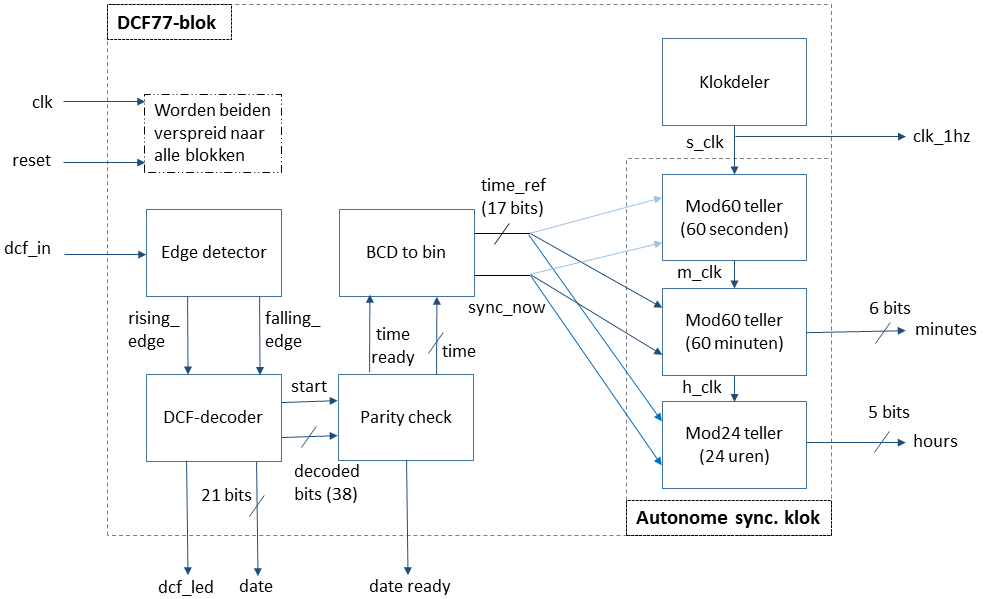
\includegraphics[keepaspectratio=true,scale=0.65]{Blokschema_DCF__Top-level_.png}
\caption{Verdeling van het DCF blok in subblokken}
\label{fig: dcf_subblokken}
\end{center}
\end{figure}


\subsection{FSM diagrammen}
Het opdelen van het grote DCF blok in subblokken is bijzonder nuttig, maar nog niet voldoende om direct een implementatie in VHDL te kunnen maken. Daarom wordt van elk voor de subblokken een FSM diagram gemaakt, waarin globaal wordt aangegeven wat er wanneer dient te gebeuren binnen elk van deze blokken. Er zijn in totaal zeven verschillende subblokken te ontwerpen, wat betekent dat er ook zeven verschillende FSM diagrammen dienen te worden getekend. Het belangrijkste en minst triviale subblok van de zeven is die van de DCF decoder. Daarom wordt hier het FSM van dit subblok besproken en worden de FSM diagrammen van de andere subblokken opgenomen in de appendices als \cref{fig: BCD2bin}, \cref{fig: edge_detector}, \cref{fig: klokdeler}, \cref{fig: mod24_teller}, \cref{fig: mod60_teller} \& \cref{fig: parity_check}.\\\\
\noindent In \cref{fig: decoder} is het FSM van de DCF decoder weergegeven. Zoals te zien is begint de decoder na reset altijd in de idle state. In deze state wordt gecontroleerd of er een nieuwe rising edge is in het DCF77 signaal en of er een nieuwe minuut is begonnen. Deze twee functies hangen nauw met elkaar samen. Immers, als er voor een bepaalde tijd geen nieuwe rising edge wordt onvangen \'en er al 59 bits zijn ontvangen, is er immers een nieuwe minuut begonnen. In de idle state wordt daarom logischerwijs geteld. Wanneer een rising edge gedetecteerd wordt, zal de tellerwaarde worden gereset, zodat dezelfde teller kan worden gebruikt om de breedte van de puls te bepalen. Wanneer een nieuwe minuut wordt gedetecteerd, zal de opslag worden leeggemaakt voor de nieuw te ontvangen bits en zal een signaal hoog worden gemaakt wat aangeeft dat er met de `oude' bits kan worden verdergewerkt. Bij iedere rising edge van het DCF77 signaal zal de DCF decoder ten slotte naar de state rising gaan.\\
\noindent In de state rising wordt, door middel van tellen, gecontroleerd of de ontvangen rising edge daadwerkelijk bij een puls uit het DCF77 signaal hoort. Is dit niet het geval, dan gaat de DCF decoder terug in de state idle en wacht op de volgende rising edge. Is dit wel het geval, dan zal er gewoon worden doorgeteld in de volgende state: dcf\_high.\\
\noindent In de state dcf\_high wordt vervolgens gekeken of de gedetecteerde DCF77 puls een 1 of een 0 codeert. Dit gebeurt door te tellen totdat er een falling edge is de binnen de marges valt van een puls van 100 ms of een puls van 200 ms. Wanneer een dergelijke falling edge is gevonden, wordt de 1 of 0 toegevoegd aan de vector met ontvangen bits en wordt het aantal ontvangen bis met 1 verhoogd. Ook het debug signaal ``led'' wordt vanuit deze state aangestuurd. Wanneer een 1 of 0 is opgeslagen, zal de DCF decoder naar de state falling gaan.\\\\
\noindent In de state falling zal de DCF decoder ten slotte de tellerwaarde weer op nul zetten. Ook het eventuele signaal dat er een nieuwe minuut is begonnen wordt weer op nul gezet. Vervolgens zal de DCF decoder weer teruggaan naar de state idle en wachten op de volgende rising edge. De cirkel is nu rond.

\begin{figure}[ht]
\begin{center}
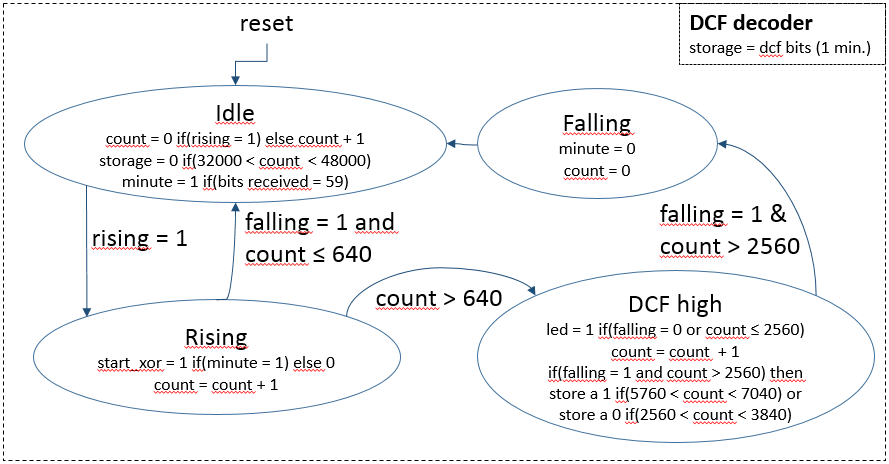
\includegraphics[keepaspectratio=true,scale=0.75]{FSM_Decoder.PNG}
\caption{FSM van het subblok decoder}
\label{fig: decoder}
\end{center}
\end{figure}

\subsection{VHDL code}
Met behulp van de FSM diagrammen kan nu behavioural VHDL worden geschreven, welke vervolgens met behulp van structural VHDL aan elkaar kan worden gehangen tot het DCF blok. Omdat het hier om een grote hoeveelheid code gaat, zijn deze bestanden opgenomen als \cref{lst: toplevel}, \cref{lst: edgedetector}, \cref{lst: decoder}, \cref{lst: paritycheck}, \cref{lst: bcd2bin}, \cref{lst: mod60teller}, \cref{lst: mod24teller}, \cref{lst: klok} \& \cref{lst: klokdeler}.

\section{Resultaten}
Aan de resultaten wordt nog gewerkt.

\section{Appendices}
\subsection{FSM BCD2bin}
\begin{figure}[ht]
\begin{center}
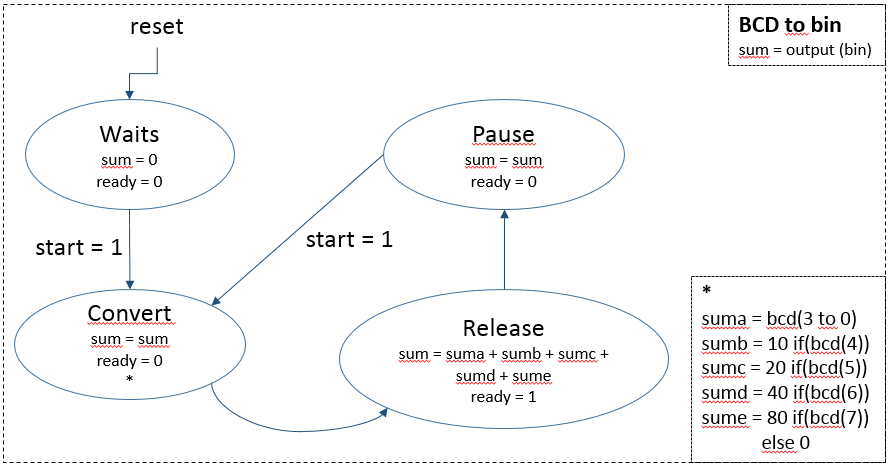
\includegraphics[keepaspectratio=true,scale=0.75]{FSM_BCD_to_bin.png}
\caption{FSM van het subblok BCD to bin}
\label{fig: BCD2bin}
\end{center}
\end{figure}

\subsection{FSM edge detector}
\begin{figure}[ht]
\begin{center}
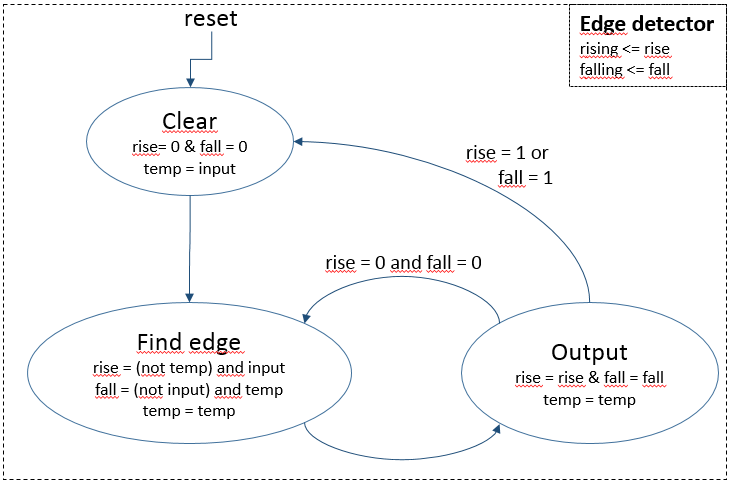
\includegraphics[keepaspectratio=true,scale=0.88]{FSM_Edge_detector.png}
\caption{FSM van het subblok edge detector}
\label{fig: edge_detector}
\end{center}
\end{figure}

\newpage
\subsection{FSM klokdeler}
\begin{figure}[ht]
\begin{center}
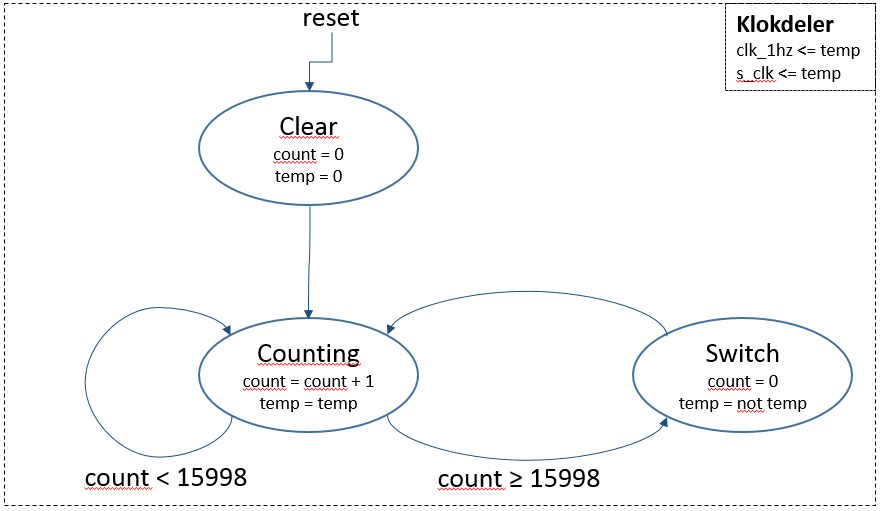
\includegraphics[keepaspectratio=true,scale=0.75]{FSM_Klokdeler.png}
\caption{FSM van het subblok klokdeler}
\label{fig: klokdeler}
\end{center}
\end{figure}

\subsection{FSM mod24 teller}
\begin{figure}[ht]
\begin{center}
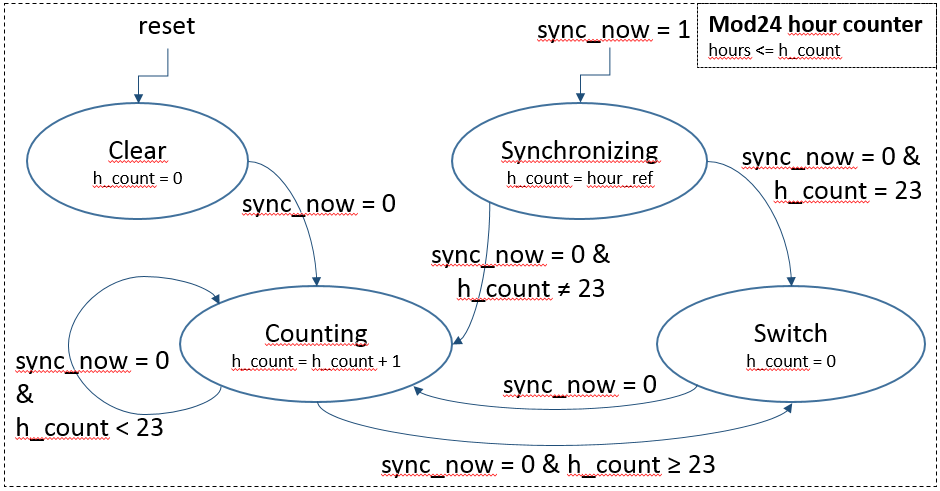
\includegraphics[keepaspectratio=true,scale=0.7]{FSM_Mod24_hour_counter.png}
\caption{FSM van het subblok mod24 teller}
\label{fig: mod24_teller}
\end{center}
\end{figure}

\newpage
\subsection{FSM mod60 teller}
\begin{figure}[ht]
\begin{center}
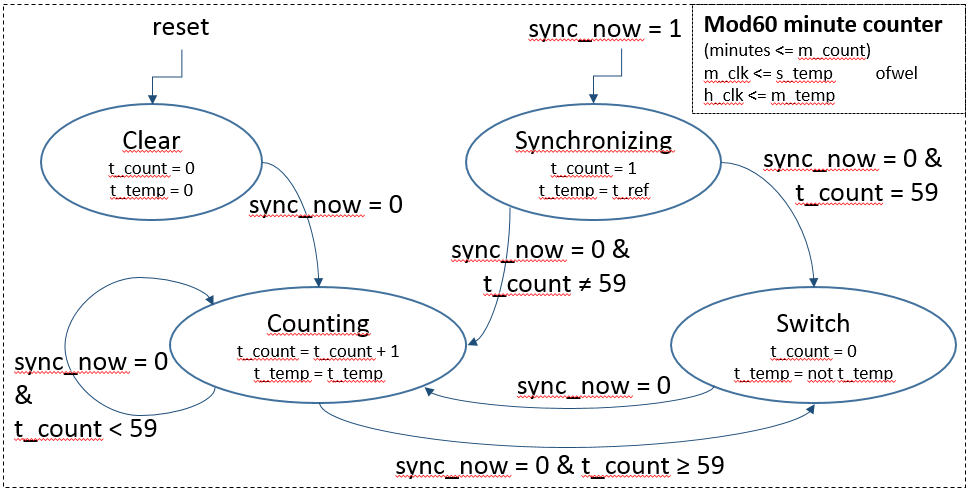
\includegraphics[keepaspectratio=true,scale=0.7]{FSM_Mod60_min__and_sec__counter.png}
\caption{FSM van het subblok mod60 teller}
\label{fig: mod60_teller}
\end{center}
\end{figure}

\subsection{FSM parity check}
\begin{figure}[ht]
\begin{center}
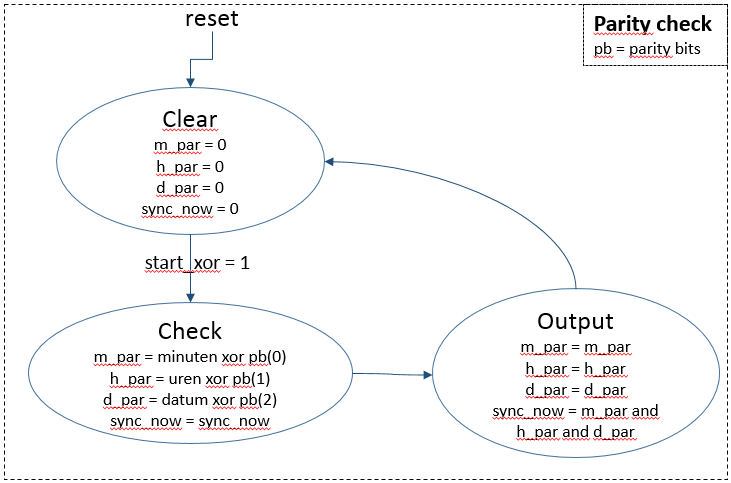
\includegraphics[keepaspectratio=true,scale=0.9]{FSM_Parity_check.png}
\caption{FSM van het subblok parity check}
\label{fig: parity_check}
\end{center}
\end{figure}

\newpage
\subsection{DCF Top-level (Structural VHDL)}
\label{lst: toplevel}
\lstinputlisting[style = VHDL]{DCF77_entity.vhdl}
\hrule
\lstinputlisting[style = VHDL]{DCF77_structure.vhdl}

\newpage
\subsection{Edge detector (Behavioural VHDL)}
\label{lst: edgedetector}
\lstinputlisting[style = VHDL]{Edge_detector_entity.vhdl}
\hrule
\lstinputlisting[style = VHDL]{Edge_detector_behaviour.vhdl}

\newpage
\subsection{Decoder (Behavioural VHDL)}
\label{lst: decoder}
\lstinputlisting[style = VHDL]{DCF_decoder_entity.vhdl}
\hrule
\lstinputlisting[style = VHDL]{DCF_decoder_behaviour.vhdl}

\newpage
\subsection{Parity check (Behavioural VHDL)}
\label{lst: paritycheck}
\lstinputlisting[style = VHDL]{Parity_check_entity.vhdl}
\hrule
\lstinputlisting[style = VHDL]{Parity_check_behaviour.vhdl}

\newpage
\subsection{BCD to bin (Behavioural VHDL)}
\label{lst: bcd2bin}
\lstinputlisting[style = VHDL]{BCD2bin_entity.vhdl}
\hrule
\lstinputlisting[style = VHDL]{BCD2bin_behaviour.vhdl}

\newpage
\subsection{Mod60 teller (Behavioural VHDL)}
\label{lst: mod60teller}
\lstinputlisting[style = VHDL]{Mod60_teller_entity.vhdl}
\hrule
\lstinputlisting[style = VHDL]{Mod60_teller_behaviour.vhdl}

\newpage
\subsection{Mod24 teller (Behavioural VHDL)}
\label{lst: mod24teller}
\lstinputlisting[style = VHDL]{Mod24_teller_entity.vhdl}
\hrule
\lstinputlisting[style = VHDL]{Mod24_teller_behaviour.vhdl}

\newpage
\subsection{Klok (Structural VHDL)}
\label{lst: klok}
\lstinputlisting[style = VHDL]{Autosyncklok_entity.vhdl}
\hrule
\lstinputlisting[style = VHDL]{Autosyncklok_structure.vhdl}

\newpage
\subsection{Klokdeler (Behavioural VHDL)}
\label{lst: klokdeler}
\lstinputlisting[style = VHDL]{Klokdeler_entity.vhdl}
\hrule
\lstinputlisting[style = VHDL]{Klokdeler_behaviour.vhdl}

\end{document}